\documentclass{article}
\usepackage{ctex}
\usepackage{fancyhdr}
\usepackage[table]{xcolor}
\usepackage{listings}
\usepackage{graphicx}
\usepackage{tikz}
\usetikzlibrary{positioning, shapes.geometric}
\usepackage{tikz-qtree}
\usepackage{hyperref}

\begin{document}
\pagestyle{fancy}
\title{接口说明}
\author{Krxk}
\date{\today}
\maketitle

\lstset{breaklines=true,keywordstyle=\color{blue},language=Python,columns=flexible,frame=single,backgroundcolor=\color{white},showspaces=false,showstringspaces=false,basicstyle=\ttfamily,commentstyle=\color{teal},stringstyle=\color{purple}}

本文档将对类接口作简要说明。
\tableofcontents
\newpage
\section{类的层次结构}
代码可在\emph{https://github.com/KrxkGit/SVRemmendation}获取,可在git中
\begin{lstlisting}
    git clone https://github.com/KrxkGit/SVRemmendation.git
\end{lstlisting}
以获取源码。

\begin{center}
    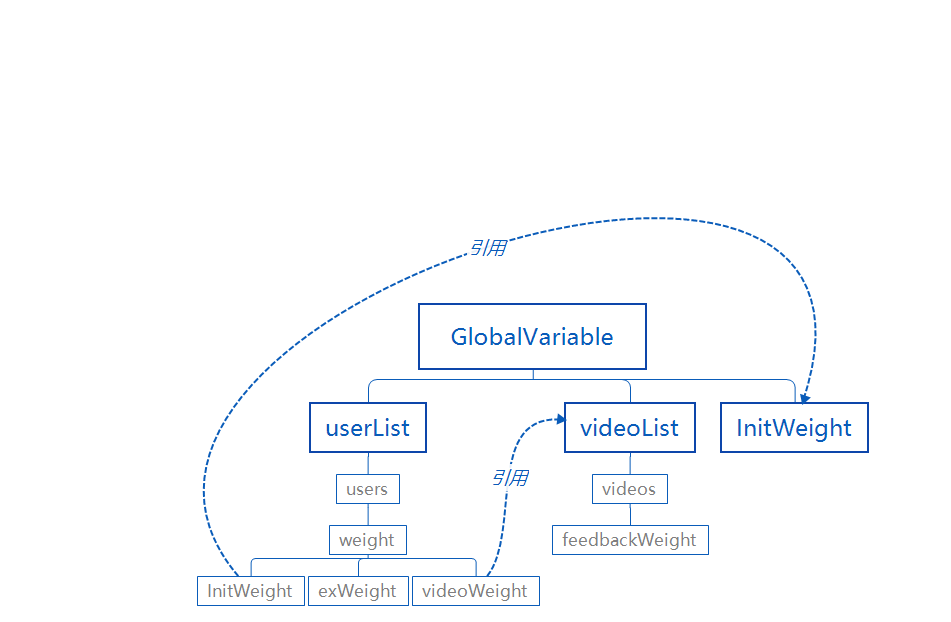
\includegraphics[scale=0.8]{../类结构.png}
\end{center}

\part{重要接口说明}
本部分某些接口需要\textcolor{red}{手动调用},需要重点关注。另外由于id是python关键字,变量"id"请替换为"uid"。
\section{GlobalVaribale}
该类负责管理所有数据,包括用户、视频
\begin{lstlisting}
class GlobalVariable:
    def __init__(self):
        self.GlobalVideoList = []   # 保存所有视频,元素为Video对象
        self.GlobalUserList = []    # 保存所有用户,元素为User对象
        self.InitWeight = InitWeightMatrix.InitWeight()  # 保存全局性的初始权重

    def GetTotalUserCount(self):  # 获得用户总数
    
    def GetTotalVideoCount(self): # 获取视频总数
        
    def add_video_to_list(self, video):
        
    def add_user_to_list(self, user):
        
    def del_video_from_list(self, video):
       
    def del_user_from_list(self, user):

    @staticmethod
    def set_video_hot(video, bSet=True):  # 设置视频视为为热,默认调用设为热

    def get_video_list_by_category(self, category):  # 返回某一类别的视频列表

    def get_user_list_by_attr(self, work_phase, gender, job):  # 根据指令用户属性返回用户列表



global_obj = GlobalVariable()  # 全局变量
refresh_frequency = 100  # 用户刷n条视频后重新计算权重
hot_add_weight_percent: float = 0.1  # 对于被设置为“热”的视频,以百分比方式增加权重,如原来权重为3,则增加为3*(1+0.1)=3.3
\end{lstlisting}

\begin{enumerate}
    \item 程序运行后,\textcolor{blue}{global\_obj}被初始化,用于管理全局信息,增加/删除 用户/视频 后需调用类中 add\_* 与 del\_*函数。文件读写操作后还需\textcolor{red}{手动调用}globao\_obj函数以更新全局管理信息。
    \item global\_obj.InitWeight 保存了初始权重对象
    \item set\_video\_hot 函数可用于\textcolor{red}{手动}将某些视频设为热度视频,可考虑结合用户界面使用
    \item get\_video\_list\_by\_category 可根据指定视频类别获取视频列表,作为用户界面辅助函数
    \item get\_user\_list\_by\_attr 可根据指定用户属性获取用户列表,作为用户界面辅助函数
    \item refresh\_frequency 表明用户在刷多少条视频后,程序重新计算初始权重表,引入该变量是为了减轻频繁更新初始权重表伴随的巨大计算量造成的负担,该变量同时也指定了某用户待播放视频列表的大小。即:其中引入了Numpy对象以加快速度。
    \item \textcolor{blue}{HelpRefreshWeight用于重新计算权重,由于该函数复杂度较高,建议放在其他线程中运行,等待计算完成后再返回,此时另一线程(该线程等待正在计算权重的工作线程完成)调用RefreshWeight以更新待播放列表。可以考虑在播放了播放列表的90\%的视频左右开始重新计算。}
    \begin{lstlisting}
class User:
    # 创建新用户
        ...
        self.to_play_list = np.zeros(refresh_frequency)  # 放置即将播放的视频
        ...
        def HelpRefreshWeight(self): 重新计算权重,作为临时结果保存起来
        def RefreshWeight(self):  # 刷新播放列表
    \end{lstlisting}
\end{enumerate}

\section{InitWeightMatrix}
\begin{lstlisting}
class InitWeight:
    def __init__(self):
        import numpy as np
        # 权重张量格式(统计性):[维度1表,维度2表,维度3表],为加快速度,表用二维数组实现
        self.weight1 = np.zeros((10, 5))
        self.weight2 = np.zeros((10, 2))
        self.weight3 = np.zeros((10, 6))
        self.weightList = [self.weight1, self.weight2, self.weight3]

    def UpdateInitWeight(self, category, work_phase, gender, job):  # 手动更新初始权重
\end{lstlisting}

\begin{enumerate}
    \item 类中weightList保存了初始权重表,利用该表可获得不同人群对不同类别视频的偏好程度,该信息可呈现在\textcolor{blue}{程序管理后台用户界面}中。
    \item UpdateInitWeight用于更新全局初始权重表,当视频被有效播放(如超过最短播放时长),请调用该函数\textcolor{red}{手动更新}全局初始权重表。
\end{enumerate}

\part{其余接口说明}
\section{Weight}
作为外壳类使用,提供权重计算功能,该类统管了InitWeight、exWeight、FreebackWeight的计算。初始化该类对象需传入用户对象(user对象)以初始化其内部的exWeight。

为了调用Weight.CalWeight以计算权重(权重由用户、视频同时索引),需额外传入视频对象(video对象)

\begin{tikzpicture}
    \Tree
    [.Weight [.InitWeight ] [.exWeight ] [.FreebackWeight ]]
\end{tikzpicture}

\section{exWeight}
根据用户历史习惯计算额外权重,该权重针对某一用户。

\section{FeedbackWeight}
该类根据视频观看、点赞率、评论率、分享率计算反馈权重。

\section{User}
用户信息类
\begin{lstlisting}
# 工作阶段(维度1)
# 0-小学生,1-初中生,2-高中生,3-大学生,4-已参加工作
work_phase: int = None
# 性别 (维度2)
# 0-男,1-女
gender: int = None
# 职业(维度3)
# 0-老师,1-学生,2-程序员,3-工程师,4-网络主播,5-其他
job: int = None
# uid
uid: int = None
# 观看视频总数
num_of_video: int = 0
# 权重计算对象
weight_obj: Weight.Weight
# 即将播放的视频列表
to_play_list   
\end{lstlisting}

\section{Video}
视频信息类
\begin{lstlisting}
# 视频类别:0-9,分别对应电视、电影,……
category: int = None
# 视频id
uid: int = None
# 视频时长
length: float = None
# 视频标题
name: str = None
# 点赞数
like: int = 0
# 评论数
comment: int = 0
# 分享数
share: int = 0
# 观看数
watch: int = 0
# 今日热点(0-否,1-是) 或者热度分级?
hot: int = 0
# 已观看用户信息[
#    [uid,次数times,平均停留时长占比ave_len_p]
#    [],...
#   ]

#播放过该视频的用户列表
user_list = []
\end{lstlisting}

\end{document}